\chapter{Implementación}

Para la realización de esta práctica se ha optado por utilizar el
lenguaje de programación \texttt{Python} mediante la librería
\href{http://lucene.apache.org/pylucene/}{\texttt{PyLucene}}. Dicha
librería lo que hace es mediante \texttt{jcc} crear un envoltorio
\emph{(wrapper)} de \texttt{Lucene} que puede ser invocado desde
\texttt{Python}. La librería \texttt{PyLucene} no es un desarrollo tan
activo y con tanta documentación como el propio \texttt{Lucene}por lo
que para usar muchas cosas se ha tenido que indagar en el propio código
fuente y a base de prueba y error.


\subsection{Instalación de PyLucene}

Para el despliegue se ha provisionado una máquina Ubuntu 16.04 LTS en \textbf{AWS}. Para la compilación de \textit{PyLucene} ha sido necesario una máquina bastante potente con al menos 2GB de memoria RAM, pero una vez compilado \textit{PyLucene} se ha podido cambiar el tipo de instancia a una t2.micro con solo 0.5GB de RAM.

\subsubsection{Instalación de dependencias}
\begin{lstlisting}
sudo apt-get update
sudo apt-get install -y ant g++ python-dev python-setuptools python-pip default-jdk-headless
sudo pip install --upgrade pip
sudo pip install setuptools --upgrade
\end{lstlisting}

\subsubsection{Descarga y extracción de `PyLucene`}
\begin{lstlisting}
wget http://apache.rediris.es/lucene/pylucene/pylucene-4.10.1-1-src.tar.gz
tar -zxvf pylucene-4.10.1-1-src.tar.gz
\end{lstlisting}

\subsubsection{Compilación e instalación de `jcc`}
\begin{lstlisting}
cd pylucene-4.10.1-1/jcc
sed -i s/java-7-openjdk-amd64/java-8-openjdk-amd64/ setup.py
python setup.py build
sudo python setup.py install
cd ..
\end{lstlisting}

\subsubsection{Edición del `Makefile` de `PyLucene`}
\begin{lstlisting}
# Linux     (Ubuntu 11.10 64-bit, Python 2.7.2, OpenJDK 1.7, setuptools 0.6.16)
# Be sure to also set JDK['linux2'] in jcc's setup.py to the JAVA_HOME value
# used below for ANT (and rebuild jcc after changing it).
PREFIX_PYTHON=/usr
ANT=JAVA_HOME=/usr/lib/jvm/java-8-openjdk-amd64 /usr/bin/ant
PYTHON=$(PREFIX_PYTHON)/bin/python
JCC=$(PYTHON) -m jcc --shared
NUM_FILES=8
\end{lstlisting}

\subsubsection{Compilación e instalación de `PyLucene`}
\begin{lstlisting}
make
sudo make install
\end{lstlisting}


\subsection{Desarrollo de los programas requeridos}

\subsubsection{Indexador}

Se ha desarrollado un indexador básico utilizando la clase
\texttt{SpanishAnalyzer}, el mayor problema encontrado a la hora de
utilizar dicha clase ha sido para indicarle la lista de palabras a
ignorar, ya que esperaba un tipo de dato especial, tras muchas pruebas se ha resuelto utilizando la clase \texttt{CharArraySet}. 

Para parsear los ficheros XML se ha utilizado la librería \texttt{etree} \href{https://docs.python.org/2/library/xml.etree.elementtree.html}{The ElementTree XML API} haciendo uso de XPath para facilitar el extraer elementos del arbol DOM.

Se ha mejorado el ejemplo proporcionado agregando más elementos de los XML como pueden ser: \textbf{tipo sesion}, \textbf{organo}
\textbf{presidente}, \textbf{fecha}, y \textbf{tipo epigrafe}.



\subsubsection{Motor de búsqueda}

Se ha desarrollado un motor de búsqueda que mediante el micro framework \texttt{Flask} expone una web que nos permite realizar búsquedas de una forma sencilla e intuitiva como se puede ver en las siguientes capturas.

Se ha utilizado \texttt{Bootstrap} para darle un mejor aspecto visual, además se ha agregado una funcionalidad para resaltar en el texto la cadena buscada.

En el caso de que se devuelvan muchos resultado solo se muestran los 10 primeros para evitar sobrecargar al servidor.

\begin{figure}
\centering
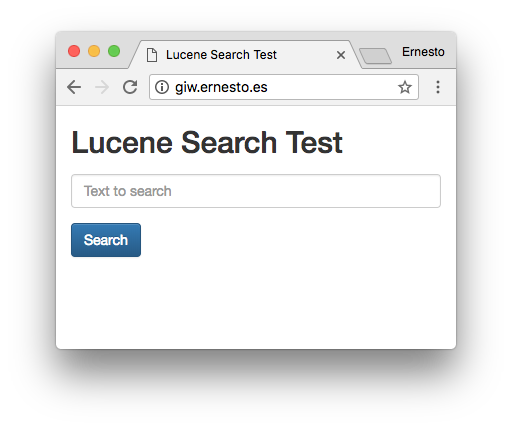
\includegraphics[width=1.0\textwidth]{../images/interface1.png}
\caption{Interfaz}
\end{figure}

\begin{figure}
\centering
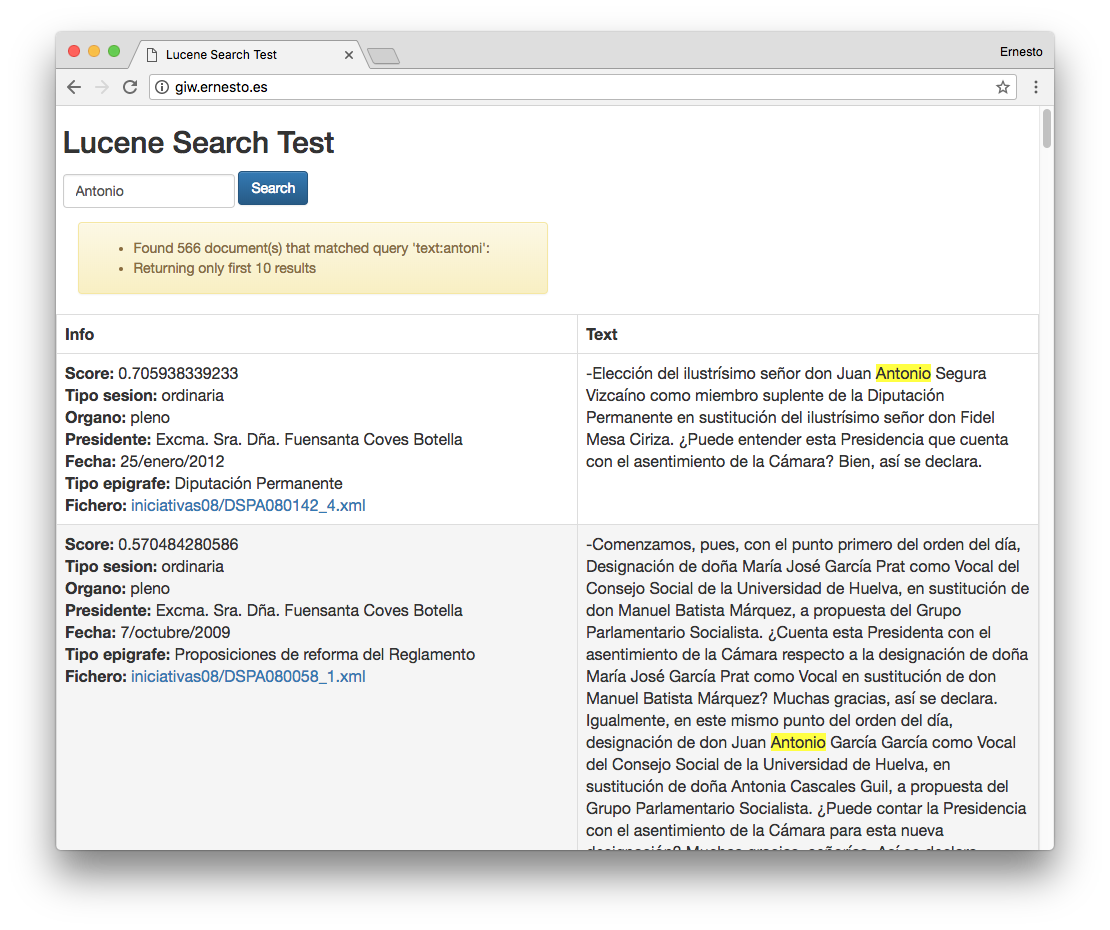
\includegraphics[width=1.1\textwidth]{../images/results1.png}
\caption{Resultados}
\end{figure}







